\documentclass[12pt]{article}
\usepackage{cwilliams-standard}

\setclass{\IPD}
\settitle{Homework 3}

\begin{document}

\maketitlepage

\section{Refinement}

From the question, I am interpretting the question to mean that we need to
track scores from previous games and continue to store them for the player to view
at later times, not single game scores viewable at the end of that game.

\textbf{Initial Feature Creation}
\begin{itemize}
    \item Scores need to be calculated at the end of the game + Scores must be stored in a database
    \item Scores must be linked to the player/user
    \item Limit number of scores stored? Prevent an overflow of data by active players
    \item Type of card game can change the score that is stored
    \item System stores game results with player details
\end{itemize}

\textbf{First Refinement}
\begin{itemize}
    \item Scores calculated at the end of the game must be saved
    \item Scores need to be saved in a database, linked to the respective players
    \item Scores will be viewable after games and show their score and their opponents scores
    \item Scores will be shown in increments of 20 on pages and will be shown when accessed instead of loading all scores at once.
    \item Data model: game session contains data, game type, players, scores, winner
    \item Users can view paginated history (20 per page)
    \item Store last 1 year of games per user
    \item Users can filter by date range or game type
\end{itemize}

\textbf{Second Refinement}
\begin{lstlisting}[language=Python]
    class match
        array details[score]
        int match_number
        def save_to_database
            send to database
            store in database
            key is match_number, value is details array
        def return_match
            return details array

    match.return_match(x)
\end{lstlisting}

\textbf{Third Refinement}

Need to entirely overhaul second refinement. Seems I entirely forgot to include... any of my specifications. 
I am also going to ditch the "match" idea instead for "GameResult" which is more descriptive and more comprehensive.

\begin{lstlisting}[language=Python]
    class GameResult:
        game_id(unique identifier)
        timestamp
        game_type (string)
        players[] (array of player objects)
        scores[] (array parallel to players)
        winner_id
    
    class ScoreTracker:
        def save_game (game_result):
            validate game_result
            assign game_id = generate_unique_id()
            assign timestamp = current_time()
            database.insert(game_result)
            if not validate(game_result):
                return error
            return game_id
        def get_user_history(user_id, page_number, page_size=20, game_type=None, date_range=None):
            offset = (page_number - 1) * page_size
            results = database.query(
                WHERE user_id IN players
                AND (game_type = game_type OR game_type IS NULL)
                AND (timestamp BETWEEN date_range OR date_range IS NULL)
                ORDER BY timestamp DESC
                LIMIT page_size
                OFFSET offset
            )
            return results
        def cleanup_old_games():
            cutoff_date = current_date - 1_year
            database.delete(WHERE timestamp < cutoff_date)
\end{lstlisting}

\textbf{Difficulties}:
\begin{itemize}
    \item Must handle high data volume (limit retention period)
    \item Performance: don't load high amounts of data (pagination is necessary)
\end{itemize}

\section{Office Generation Modules}

\begin{figure}[H]
    \centering
    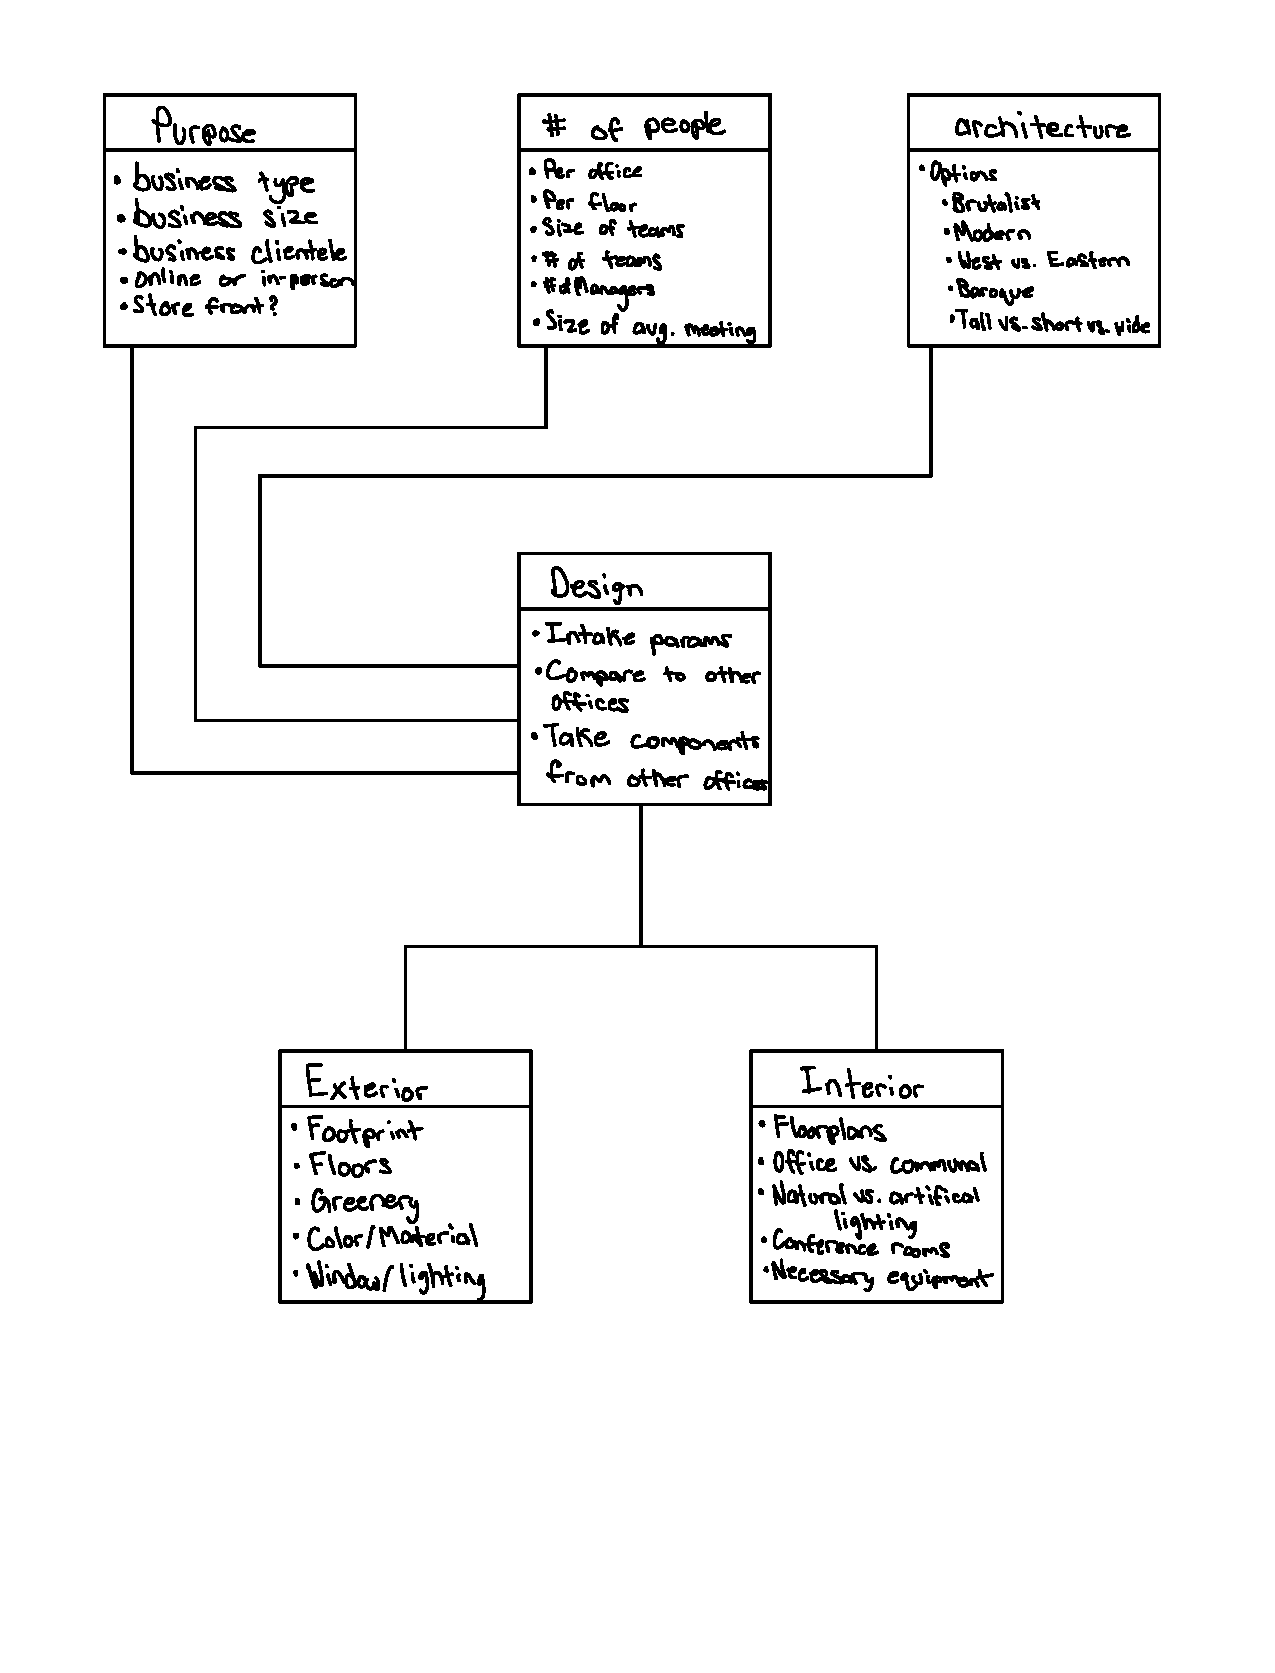
\includegraphics[width=0.75\linewidth]{images/HW3.pdf}
    \caption{Modules for Office Generator}
    \label{fig:officegenerator}
\end{figure}

\section{Important Design Modeling Characteristic}

I believe of the 10 design characteristics we discussed, the \textbf{cohesion} is the most important. High cohesion ensures that
each module has a single, well defined purpose with closely related functionalities grouped with it. This particular principle is
most important because it directly affects many other principles: high cohesion is easier to understand (abstraction),
easier to maintain (modularity), and better at hiding implementation details (encapsulation).
\section{Old vs. New Requirement Capturing}

The older version of requirement capturing placed a heavy emphasis on the customer being the source of the issues, where the customer creates requirements 
or boundaries that don't make sense within the context of the project because they lack understanding about the topic. In contrast, the new version offers philosophical statements like "we don't understand everything about the world," 
which, while universally true, provides no actionable guidance on identifying which stakeholder has the problem or how to prevent common requirement traps.
The older model describes when customers are the root of ambigious or vague requirements that are a common trap which lead teams to fall into metaphorical potholes and having to go back to the drawing board. 

\section{"More Than Code"}

I believe the model presented by Ramin et al. represents a strong improvement over previous contribution models because it acknowledges
non-technical contributions that often go overlooked. However, the model has limitations as well. By only basing their work off of the 2017 Scrum Guide,
the authors only present a "vanilla Scrum", which likely misses some real world adaptations that teams like to make to the Scrum format. Also,
some contributions like 'Product Backlog Maintenance' get addressed organically through the processes of development, reducing the distinctiveness of the model. 

The \textit{Team Contribution Analysis} use case is very effective because, using Table 2's contribution list, teams can identify "project
contributions that have been previously overlooked [Ramin et al.]." This helps to alleviate a problem that many teams face which is that developers spend a minority
of their time actually coding/programming. This leaves many essential and necessary contributions unrecognized like backlog refinement and impediment removal.
Also, it directly supports the Scrum ideology of transparency and self-organization because team members can communicate and air misunderstandings
easier which creates opportunities for clarification instead of allowing confusion and grievances to fester.

\end{document}